\chapter{Thread}

\section{Introduzione}

\dfn{Thread}{
    Il Thread è un flusso sequenziale di controllo (esecuzione di istruzioni) in
    un programma. Un programma può avere più thread che eseguono
    contemporaneamente (in modo concorrente). Tutti i thread di un
    programma condividono lo stesso spazio di indirizzamento\footnote{A differenza dei processi}.    
}

\nt{Un thread può essere visto come un light-weight process.}

\dfn{Classe Thread}{
    La classe Thread è una classe Java che permette di creare e gestire
    thread. La classe Thread ha un costruttore che prende un oggetto
    Runnable come parametro. Runnable è un'interfaccia che ha un
    solo metodo run() che deve essere implementato. Il metodo run()
    contiene il codice che deve essere eseguito dal thread.

}

\cor{API della classe Thread}{
    \begin{itemize}
        \item [$\Rightarrow$] start() - avvia il thread;
        \item [$\Rightarrow$] run() - contiene il codice che deve essere eseguito dal thread;
        \item [$\Rightarrow$] sleep(int ms) - sospende il thread per ms millisecondi;
        \item [$\Rightarrow$] join() - attende la terminazione del thread;
        \item [$\Rightarrow$] isAlive() - ritorna true se il thread è in esecuzione;
        \item [$\Rightarrow$] getName() - ritorna il nome del thread;
        \item [$\Rightarrow$] setName(String name) - imposta il nome del thread.
    \end{itemize}

}

\nt{Lo stato Runnable indica che il thread è pronto per essere eseguito (non necessaria
mente in esecuzione).}

\dfn{Interface Runnable}{
    L'interfaccia Runnable è un'interfaccia Java che ha un solo metodo
    run() che deve essere implementato. Il metodo run() contiene il
    codice che deve essere eseguito dal thread.

}

\dfn{Join}{
    Il metodo join() permette di attendere la terminazione del thread su cui
    è invocato. Il thread che invoca il metodo join() viene sospeso fino a
    quando il thread su cui è invocato non termina.

}

\nt{Il metodo join() va invocato \underline{dopo} il metodo start() e deve
essere invocato con il meccanismo try/catch.}

\begin{figure}
    \centering
    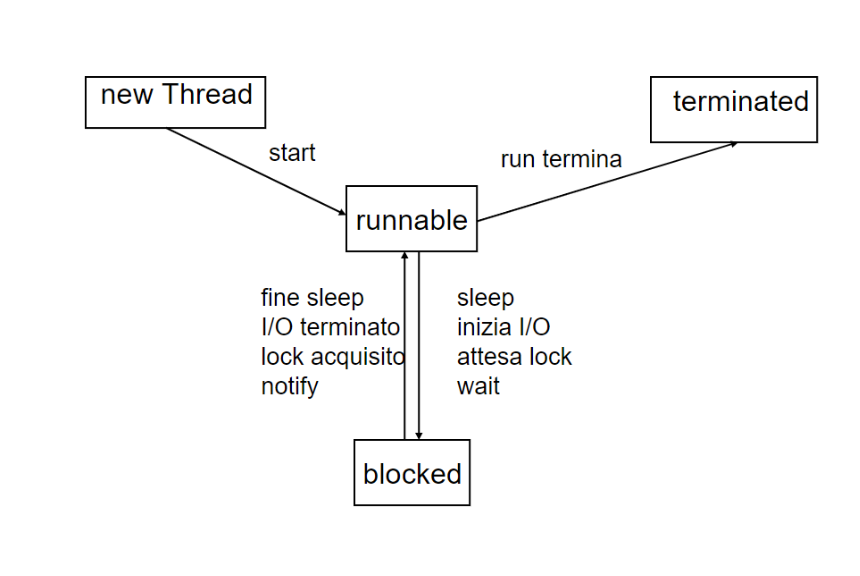
\includegraphics[scale=0.5]{images/thread/Ciclo di vita.png}
    \caption{Ciclo di vita di un thread}
    \label{fig:Thread}
\end{figure}

\section{Thread in Java}

\dfn{Semaphore}{La classe Semaphore è stata introdotta per aiutare chi aveva programmato in C.
Semaphore(int n) è un semaforo con n permessi. Possiede i metodi:
\begin{itemize}
    \item acquire() - prende un permesso;
    \item release() - rilascia un permesso.
\end{itemize}
}

\nt{Ogni oggetto ha un proprio lock: un semaforo binario con una lista che, se utilizzato, blocca gli accessi
concorrenti garantendo la mutua esclusione. Lo scheduler del lock ha una propria politica di gestione.}

\dfn{Sincronizzazione}{
Per ogni classe Java è possibile definire dei metodi synchronized. Quando un thread invoca un metodo
synchronized, il thread acquisisce il lock dell'oggetto su cui è invocato il metodo. La sintassi è:
public synchronized void metodo() \{...sezione critica...\}

}

\section{Sincronizzazione lato server e lato client}

\dfn{Sincronizzazione lato server}{
\begin{itemize}
    \item [$\Rightarrow$] L'oggetto protegge le variabili condivise e offre metodi
    synchronized per operare su di esse per cui si auto-
    protegge dagli accessi esterni;
    \item [$\Rightarrow$] I client, invocando metodi synchronized sull'oggetto
    condiviso, automaticamente si sincronizzano
    nell'accesso all'oggetto stesso;
    \item [$\Rightarrow$] imitazioni: definire synchronized i metodi dell'oggetto
    potrebbe non essere sufficiente per sincronizzare le
    attività dei thread.
\end{itemize}
}

\dfn{Sincronizzazione lato client}{
\begin{itemize}
    \item [$\Rightarrow$] L'oggetto non viene protetto da accessi paralleli;
    \item [$\Rightarrow$] Tutti i client di un oggetto condiviso accedono all'oggetto
    attraverso blocchi sincronizzati sul lock dell'oggetto
    stesso;
    \item [$\Rightarrow$] Limitazioni: se un client non implementa correttamente
    gli accessi all'oggetto condiviso si ottiene un
    malfunzionamento;
    \item [$\Rightarrow$] Ma talvolta è necessario implementare la mutua
    esclusione in questo modo.
\end{itemize}
}

\cor{Cooperazione tra thread}{
    \begin{itemize}
        \item \texttt{wait()} - sospende il thread corrente e rilascia il lock dell'oggetto su cui è invocato;
        \item \texttt{notify()} - risveglia un thread sospeso su un oggetto;
        \item \texttt{notifyAll()} - risveglia tutti i thread sospesi su un oggetto.
    \end{itemize}
}

\nt{Generalmente conviene usare \texttt{notifyAll()} per evitare che un thread venga risvegliato e poi
rimesso in attesa (causando un deadlock).}

\dfn{BlockingQueue}{
    BlockingQueue è un'interfaccia Java che estende l'interfaccia Queue. BlockingQueue
    ha i metodi put() e take() che permettono di inserire e rimuovere elementi dalla coda.
    BlockingQueue è una coda sincronizzata: se la coda è vuota, il metodo take() sospende il
    thread finché non viene inserito un elemento nella coda. Se la coda è piena, il metodo put()
    sospende il thread finché non viene rimosso un elemento dalla coda.
}

\nt{Un'implementazione di BlockingQueue è la classe ArrayBlockingQueue.}

\subsection{Librerie}

\dfn{ReentrantLock}{
    La classe ReentrantLock è una classe Java che ha i metodi lock() e unlock() che permettono
    di acquisire e rilasciare il lock. La classe ReentrantLock ha anche i metodi tryLock() e
    tryLock(long timeout, TimeUnit unit) che permettono di acquisire il lock se è disponibile
    e di rilasciarlo se non è disponibile entro il timeout specificato.
}

\cor{Lock e Condition}{
    La classe Lock è un'interfaccia Java che ha i metodi lock() e unlock() che permettono di
    acquisire e rilasciare il lock. La classe Condition è un'interfaccia Java che ha i metodi
    await() e signal() che permettono di sospendere e risvegliare un thread.
}

\dfn{ReadWriteLock}{
    La classe ReadWriteLock è un'interfaccia Java che ha i metodi readLock() e writeLock() che
    permettono di acquisire il lock in lettura e scrittura. La classe ReadWriteLock ha anche i
    metodi readUnlock() e writeUnlock() che permettono di rilasciare il lock in lettura e
    scrittura.
}

\section{Thread Pool}

\dfn{Thread e Task}{
    Task: unità logicamente indipendente di lavoro che può essere eseguita da un thread,
    in parallelo con altri task.

    Thread: flusso di controllo che esegue un task.
}

\dfn{Thread pool}{
    Un thread pool è un insieme di thread che possono essere riutilizzati per eseguire task.
    Un thread pool ha un numero massimo di thread che possono essere creati. Se tutti i thread
    sono occupati, i task vengono messi in una coda e vengono eseguiti quando un thread è
    disponibile.
}

\cor{Executor}{
    Un executor è un'interfaccia Java che ha il metodo execute(Runnable command) che permette
    di eseguire un task.
}

\paragraph{Ci sono 3 tipi di executor:}
\begin{itemize}
    \item [$\Rightarrow$] ThreadPoolExecutor: implementazione di un thread pool;
    \item [$\Rightarrow$] ScheduledThreadPoolExecutor: implementazione di un thread pool che
    permette di eseguire task in un momento specificato;
    \item [$\Rightarrow$] ForkJoinPool: implementazione di un thread pool che permette di
    eseguire task in parallelo.

\end{itemize}

\nt{La graceful degrading è una tecnica che permette di ridurre il carico di lavoro quando il
sistema è sovraccarico.}

\dfn{Callable}{
    Callable è un'interfaccia Java che ha il metodo call() che permette di eseguire un task e
    ritornare un risultato di tipo generico T.
}

\dfn{Future}{
    Future è un'interfaccia Java che ha il metodo get() che permette di ottenere il risultato
    di un task. Il metodo get() è bloccante: se il risultato non è ancora disponibile, il
    thread viene sospeso finché il risultato non è disponibile.
    Future ha anche il metodo FutureTask che crea un FutureTask che, quando parte, esegue il
    task passato come parametro. Fure offre anche il metodo isDone() che ritorna true se il
    task è completato.
}

\nt{I pool thread sono utili per evitare di creare e distruggere thread, aumentando la scalabilità.}

\dfn{Pipe}{
    Una pipe è un canale di comunicazione tra due thread. Una pipe ha un buffer che permette
    di scambiare dati tra i due thread.
}

\cor{Sender e Receiver}{
    Sender è un'interfaccia Java che ha il metodo send(Object message) che permette di
    inviare un messaggio. Receiver è un'interfaccia Java che ha il metodo receive() che
    permette di ricevere un messaggio.
}